%===============================================================================
% LaTeX sjabloon voor de bachelorproef toegepaste informatica aan HOGENT
% Meer info op https://github.com/HoGentTIN/bachproef-latex-sjabloon
%===============================================================================

\documentclass{bachproef-tin}

\usepackage{hogent-thesis-titlepage} % Titelpagina conform aan HOGENT huisstijl
\usepackage{xr}
\usepackage{pgfplots}
\usepackage{hyperref}
\usepackage[backend=biber, style=apalike, sorting=ynt]{biblatex}
\addbibresource{bachproef-tin.bib}
\usepackage[xindy, nonumberlist]{glossaries}
\newglossaryentry{SalesEnablement}
{
    name=Sales Enablement,
    description={Sales enablement is the process of providing the sales organization with the information, content and tools that help salespeople sell more effectively. }
}
\newglossaryentry{CI/CD}
{
    name=CI/CD,
    description={Continuous Integration/Continuous Delivery is a process framework Mathematics is what mathematicians do}
}
\newglossaryentry{Scrum}
{
    name=Scrum,
    description={Scrum is one of the most popular agile methodologies, based on a timeboxed iteration (sprint), with a clearly defined goal and scope. It comes with a limited set of roles and ceremonies to stay as light weight as possible.}
}
\newglossaryentry{Epic}
{
    name=Epic,
    description={At Showpad, an Epic is the unit of Customer Value delivery. The combination of all Epics forms the Roadmap. To enable a value delivery focus, we limit the scope of an Epic to typically fit in one or a maximum of two release cycles. Epics are large bodies of work that can be broken down into a number of User Stories. In an Epic, we focus on tackling 1 and only 1, clearly defined problem specific to 1 principal Actor’s (user persona) User Experience. Multiple teams can work on the same Epic. The Epic is to a Release, what a User Story is to a Sprint.
    }
}
\newglossaryentry{Userstory}
{
    name=User Story,
    description={At Showpad, User Stories are short requirements or requests written from the perspective of an end-user. A User Story fits into the timebox of a Sprint and is the lowest level of granularity for planning and delivering work. A User Story has a 1-on-1 relationship with a team that will implement it.}
}
\newglossaryentry{Sprint}
{
        name=Sprint,
        description={A sprint is a short, time-boxed period when a scrum team works to complete a set amount of work. At Showpad, a sprint is typically 2 to 3 weeks long, it is up to the Scrum team to determine the length of Sprints. once chosen, it puts the team in a fixed cadence of delivery.}
}
\newglossaryentry{Monorepo}
{
    name=Monorepo,
    description={Two dominant models for structuring code bases exist in the version control space. Monorepo and Polyrepo. In a Monorepo setup, the codebases of the multiple projects are kept together in a single repository. These projects have a well-defined relationship. The colocation of code and the well-defined relationship among the projects make a Monorepo a Monorepo.}
}
\newglossaryentry{Cycletime}
{
    name=Cycle Time,
    description={Cycle Time is the elapsed time from the start of the first task to finishing the last job to deliver 1 work item.}
}

\newacronym{CI}{CI}{Continuous Integration}
\newacronym{CD}{CD}{Continuous Delivery}
\newacronym{SAAS}{SAAS}{Software as a Service}
\newacronym{ARR}{ARR}{Annual Recurring Revenue}
\newacronym{CRM}{CRM}{Customer Relationship Management}
\newacronym{DDD}{DDD}{Domain Driven Design}

    
\makeglossaries
\usepackage{graphicx}
\graphicspath{ {./img/} }

%%---------- Documenteigenschappen ---------------------------------------------
% TODO: Vul dit aan met je eigen info:

% De titel van het rapport/bachelorproef
\title{The influence of the Micro Frontend architectural pattern on the productivity of front-end engineers working in a monorepo environment}

% Je eigen naam
\author{Simon Baeyens}

% De naam van je promotor (lector van de opleiding)
\promotor{Stefaan De Cock}

% De naam van je co-promotor. Als je promotor ook je opdrachtgever is en je
% dus ook inhoudelijk begeleidt (en enkel dan!), mag je dit leeg laten.
\copromotor{Bart Hemmeryckx-Deleersnijder}

% Indien je bachelorproef in opdracht van/in samenwerking met een bedrijf of
% externe organisatie geschreven is, geef je hier de naam. Zoniet laat je dit
% zoals het is.
\instelling{Showpad}

% Academiejaar
\academiejaar{2021-2022}

% Examenperiode
%  - 1e semester = 1e examenperiode => 1
%  - 2e semester = 2e examenperiode => 2
%  - tweede zit  = 3e examenperiode => 3
\examenperiode{3}

%===============================================================================
% Inhoud document
%===============================================================================

\begin{document}

%---------- Taalselectie -------------------------------------------------------
% Als je je bachelorproef in het Engels schrijft, haal dan onderstaande regel
% uit commentaar. Let op: de tekst op de voorkaft blijft in het Nederlands, en
% dat is ook de bedoeling!

\selectlanguage{english}

%---------- Titelblad ----------------------------------------------------------
\inserttitlepage

%---------- Samenvatting, voorwoord --------------------------------------------
\usechapterimagefalse
%%=============================================================================
%% Voorwoord
%%=============================================================================

\chapter*{\IfLanguageName{dutch}{Woord vooraf}{Preface}}
\label{ch:voorwoord}

%% TODO:
%% Het voorwoord is het enige deel van de bachelorproef waar je vanuit je
%% eigen standpunt (``ik-vorm'') mag schrijven. Je kan hier bv. motiveren
%% waarom jij het onderwerp wil bespreken.
%% Vergeet ook niet te bedanken wie je geholpen/gesteund/... heeft

During my Bachelor studies Applied Informatics, I got more and more facinated by UX design and frontend web development and decided to pursue a career in this functional domain. I was delighted as I joined Showpad for a 3 month internship, to be able to work as a frontend engineer in the CRM scrum team. The size and the complexity of the Showpad SaaS product, the importance of the user interface in providing an optimal user experience for the 250.000 users of the product, challenged me in putting in practice what I learned during my studies.

Thanks go to Bart Hemmeryckx-Deleersnijder my copromotor at Showpad, and director product engineering for the CRM team, for providing me with guidance and support on how software engineering is applied at Showpad. Special thanks to Pablo Frosi who was my front-end mentor during my internship and helped me out immensely.

Simon Baeyens, Aalst, August 2022
%%=============================================================================
%% Samenvatting
%%=============================================================================

% TODO: De "abstract" of samenvatting is een kernachtige (~ 1 blz. voor een
% thesis) synthese van het document.
%
% Deze aspecten moeten zeker aan bod komen:
% - Context: waarom is dit werk belangrijk?
% - Nood: waarom moest dit onderzocht worden?
% - Taak: wat heb je precies gedaan?
% - Object: wat staat in dit document geschreven?
% - Resultaat: wat was het resultaat?
% - Conclusie: wat is/zijn de belangrijkste conclusie(s)?
% - Perspectief: blijven er nog vragen open die in de toekomst nog kunnen
%    onderzocht worden? Wat is een mogelijk vervolg voor jouw onderzoek?
%
% LET OP! Een samenvatting is GEEN voorwoord!

%%---------- Nederlandse samenvatting -----------------------------------------
%
% TODO: Als je je bachelorproef in het Engels schrijft, moet je eerst een
% Nederlandse samenvatting invoegen. Haal daarvoor onderstaande code uit
% commentaar.
% Wie zijn bachelorproef in het Nederlands schrijft, kan dit negeren, de inhoud
% wordt niet in het document ingevoegd.

\IfLanguageName{english}{
\selectlanguage{dutch}
\chapter*{Samenvatting}
Wanneer software producten groeien in functionaliteit en omvang, en zeker wanneer het aantal ontwikkelaars dat eraan werkt toeneemt, is het van belang dat de architectuur van de software mee evolueert. In de beginfase van een software product is de keuze voor een monolitische architectuur een veel gebruikte praktijk. Maar op schaal, heeft dit architecturaal patroon een vertragend effect op het leveren van toegevoegde waarde richting gebruikers. Het minimaliseren van dit vertragend effect, is een van de redenen waarom Microservices en Micro frontend architecturale patronen winnen aan populariteit in de wereld van web toepassingen.

In deze Bachelor thesis bekijken we de invloed van het micro frontend architecturaal patroon op de productiviteit van frontend ontwikkelaars die momenteel in een monorepo omgeving werken.

Om aan te tonen dat dit concept een antwoord biedt, werd een beperkt stuk functionaliteit geisoleerd in een micro frontend applicatie en werd het effect op de bouwtijden en doorlooptijden gemeten.

Het resultaat van deze proof-of-concept blijkt postief. De bouwtijd van de ge\"{i}soleerde functionaliteit bleek vier keer korter dan bij de basis meting. De doorlooptijd van de aangepaste CI/CD pijplijn werd met 27\% gereduceerd.

De resultaten zien er alvast veelbelovend uit en toont potentieel voor het verhogen van de productiviteit van individuele ontwikkelaars en teams, zowel als een verhoogde autonomie van teams binnen een multi-team ontwikkel organisatie als Showpad.

Maar dit alles komt niet gratis. Het is geweten dat in microservice en micro frontend architecturen, de systeem complexiteit omhoog gaat vanwege het groeiend aantal componenten. Ten tweede, het opbreken van een monolitische architectuur vraagt veel werk en zal dus ook behoorlijk wat tijd vragen opdat de maximale impact zich zou materialiseren. Tot slot, is het opdelen van een monolitische architectuur niet enkel een technische uitdaging, maar vereist vooral ook een afstemming van het product domein model. Om tot deze afstemming te komen pleiten kennisleiders van microservice en microfrontend architectuur voor het toepassen van Domain Driven Development.

Een software bedrijf heeft als hoofddoel product innovatie zo snel mogelijk bij zijn klanten en gebruikers te krijgen. Binnen Showpad is het nu aan het Product \& Engineering management team om verder uit te werken of en hoe het gebruik van micro frontends een antwoord biedt op de architecturale uitdagingen die van invloed zijn op het schalen van het product, de autonomie en productiviteit van teams.
\selectlanguage{english}
}{}
%%---------- Samenvatting -----------------------------------------------------
% De samenvatting in de hoofdtaal van het document

\chapter*{\IfLanguageName{dutch}{Samenvatting}{Abstract}}
As software products grow in scope and size, especially when the number of developers working on them grows, the need to scale the architecture along is essential. In the start-up phase of a software product, choosing a monolith architecture is more or less standard practice. But at scale, this architectural pattern tends to slow teams down in delivering value to software users. Minimizing the delay in value delivery is one of the reasons Microservices and Micro frontend architecture patterns gain popularity in the web application space. 

In this bachelor thesis, the influence of the Micro Front-end architectural pattern on the productivity of frontend engineers working in a mono repo environment is evaluated. 

As a proof of concept, a small piece of the product functionality was isolated in a micro frontend application, and the effect on the build time and cycle time was measured.

The results of the proof of concepts show a positive impact. The isolated functionality's build time was four times faster than the baseline measurements. The cycle time of the adapted CI/CD pipeline for the micro frontend application was reduced by 27\%.

These results for sure look promising. It has the potential for the productivity of individual developers and teams as to the autonomy of teams in a multi-team development organization like Showpad. 

But it will not come for free. It is known that in microservice and micro frontend architectures, the system's complexity increases due to the growing number of components. Secondly, decomposing a monolith architecture requires a lot of work, and it will take time before the full impact materializes. Last but not least, decomposing a monolith architecture is not only a technical challenge but requires alignment to the product domain model. To get to this alignment, thought leaders in microservice and micro frontend architectures plea for applying Domain Driven Development as the basis.

A software company's primary purpose is to get product innovation in the hands of customers and users as soon as possible. In Showpad, it is now up to the Product \& Engineering leadership to further explore the usage of Micro frontends to answer the architectural challenges that influence scaling the product and the autonomy and productivity of teams.

%---------- Inhoudstafel -------------------------------------------------------
\pagestyle{empty} % Geen hoofding
\tableofcontents  % Voeg de inhoudstafel toe
\cleardoublepage  % Zorg dat volgende hoofstuk op een oneven pagina begint
\pagestyle{fancy} % Zet hoofding opnieuw aan

%---------- Lijst figuren, afkortingen, ... ------------------------------------

% Indien gewenst kan je hier een lijst van figuren/tabellen opgeven. Geef in
% dat geval je figuren/tabellen altijd een korte beschrijving:
%
%  \caption[korte beschrijving]{uitgebreide beschrijving}
%
% De korte beschrijving wordt gebruikt voor deze lijst, de uitgebreide staat bij
% de figuur of tabel zelf.

\listoffigures
\listoftables
%\lstlistoflistings

% Als je een lijst van afkortingen of termen wil toevoegen, dan hoort die
% hier thuis. Gebruik bijvoorbeeld de ``glossaries'' package.
% https://www.overleaf.com/learn/latex/Glossaries
\glsaddall
\printglossaries

%---------- Kern ---------------------------------------------------------------

% De eerste hoofdstukken van een bachelorproef zijn meestal een inleiding op
% het onderwerp, literatuurstudie en verantwoording methodologie.
% Aarzel niet om een meer beschrijvende titel aan deze hoofstukken te geven of
% om bijvoorbeeld de inleiding en/of stand van zaken over meerdere hoofdstukken
% te verspreiden!

%%=============================================================================
%% Inleiding
%%=============================================================================

\chapter{\IfLanguageName{dutch}{Inleiding}{Introduction}}
\label{ch:inleiding}

Software products with codebases of multiple millions of lines of code, built over more than a decade by a few hundred different software engineers, typically come with challenges of scale that far exceed the theoretical context in which software methodologies and methods are defined. Handling legacy technology stacks and architectures while further extending and evolving the product functionality comes with specific challenges. These challenges impact the productivity of product teams, individual engineers, and the business.

Instead of exploring the opportunity of a software architecture pattern as micro-frontends in isolation, it adds more value to do it in the context of a real-world product development environment. I was fortunate to conduct my internship at Showpad, which offers the perfect setting to conduct my research.
\subsection{The company: Showpad}
Showpad is one of the successful scale-ups that emerged from the Ghent tech start-up scene, founded in 2011 as a spin-off of the web agency In The Pocket. Showpad initially developed an iPad application to enable salespeople to get their job done on the road and at sales fairs by providing them with compelling online digital sales content. Due to its success,  an online back office application extended the mobile application. As sales teams grew and started to work more and more hybrid, combining field sales with selling from the office, a browser-based web application became the dominant interface for driving the company's business success.

\gls{SalesEnablement} is the business domain in which Showpad is active and where market analysts Gartner and Forrester perceive it as one of the global leaders in this space. Showpad works according to a \gls{SAAS} (Software As A Service) business model. Customers subscribe to the service paying an annual fee per user resulting in Annual Recurring Revenue growing 20\% to 30\% year over year. Showpad generates 50\% of its revenue in Europe and 50\% in the US.

Showpad celebrated its 11 anniversary in May 2022. It grew from a three-person start-up in the living room of one of the co-founders to a sizable global scale-up of 600 people with multiple offices across the globe. The product engineering team evolved from 1 engineer to a Research and Development department of more than 220 people, including 130 software engineers active in 18 scrum teams. 
\section{\IfLanguageName{dutch}{Probleemstelling}{Problem Statement}}
\label{sec:probleemstelling}
Although applied to the situation at Showpad, the challenges that set the context for this bachelor thesis are common to many fast-growing software companies.
During my internship at Showpad as a front-end engineer and member of the CRM team, I experienced several scaling challenges firsthand. Contributing to improved productivity of front-end engineers in Showpad by exploring how micro-frontend architecture can help in an enhanced ``time to value'' was a valuable path.
\subsection{Emerging Architecture}
In the early days of the venture, given the limited amount of people working on the code base, the limited functionality of the product, and the limited user base, choosing a monolith architecture was the obvious choice to make. At that time, this architectural pattern provided nothing but benefits. It led to a performant software system while keeping the complexity and the number of system components under control. In the meantime, the software system has grown to a codebase of 12 million lines of code, spread over 400+ GitLab repositories. A handful of monolith components still cover the core functionality of the \gls{SAAS} product. And the drawbacks of this once successful architecture start to hurt.
\subsection{Front-end CI/CD pipeline}
One of the monolith architectural components at Showpad is the web front-end stack. It originated from a deliberate choice to manage the front-end stack as a mono repo. With all teams contributing to the product's web user interface, all units must go through the same \gls{CI/CD} pipeline when bringing changes to production. Over the years, the performance of this \gls{CI/CD} pipeline has become a significant bottleneck slowing down teams substantially. 
Until a year ago, the success rate of bringing front-end updates to production was, on average, once every two weeks. A focussed process improvement project resulted in a structural improvement in daily deploys to production. 
Architectural changes are required to get to a higher deployment frequency. The hypothesis to be tested is whether the micro-frontends architectural pattern is a way forward in decomposing the monolith architecture.
\subsection{Growing Organisation}
The product engineering organization also snowballed to support the growing scope of the business and the product. The number of people building and maintaining the product doubled over the past three years. Impacting the complexity of the organization and the way of working; aligning on why what, and how to do things across 18 globally distributed \gls{Scrum} teams is a different ballgame than doing it with a hand full of engineers around a kitchen table in the startup's early days. 
\subsection{Impact of Scale}
There are multiple angles when evaluating the impact of scale. When narrowing down the problem statement for this thesis, we first define the 3 dominant perspectives.
\subsubsection{The Business}
From a business perspective, R\&D is essential to the investments required to run a successful business. In \gls{SAAS} businesses, this is typically around 23\% of the annual revenue. Revenue growth is a lagging indicator of the return on that investment in R\&D due to the natural lag between the moment of investment and the moment the newly built functionality is in customers' hands, generating value. So the most significant focus is on ``time to value''. In Showpad, they frame it as the time needed ``From idea till smile of the customer''. In traditional lean metrics, this is lead time. A shorter lead time means a higher impact on business.

As the company grows in size and complexity, paying attention to the productivity impact observed through ``time to value'' is a key attention point for the leadership of the R\&D organization. Showpad organizes the product roadmap in \glspl{Epic} as the top level unit of work with a targeted lead time of 2 months. \Glspl{Epic} are further decomposed in a set of User Stories which are tipically handled within a \gls{Sprint} cycle. The typical \gls{Sprint} length of 2 weeks provides a team with four iterations to deliver on an \gls{Epic}.
\subsubsection{Scrum team}
Showpad organizes its product development life cycle based on the \gls{Scrum} methodology. Currently, there are 18 \gls{Scrum} teams with over 130 engineers actively working on the Showpad \gls{SAAS} product. 
Inter-team dependencies, alignment of scope, the complexity of the software stack, the architectural reality, and the slowing down effect of a natural level of technical debt resulting from 11 years of high pace product development are critical challenges to productivity in a venture of this scale.
\subsubsection{Individual developer}
Software engineers want to spend most of their time building software and have it in the hands of users. Dependencies on other teams, processes, and architectural constraints slow the developer's productivity and reduce the developer's happiness.
\section{\IfLanguageName{dutch}{Onderzoeksvraag}{Research question}}
\label{sec:onderzoeksvraag}
What is the influence of applying the Micro Frontend architectural pattern on the productivity of frontend engineers working in a mono repo environment?

\section{\IfLanguageName{dutch}{Onderzoeksdoelstelling}{Research objective}}
\label{sec:onderzoeksdoelstelling}
As a proof of concept, we will isolate a chunk of functionality from the frontend mono repo into a micro frontend application. This way, we want to prove the positive impact of this architectural pattern on the productivity of the frontend engineers and their teams.
We will measure the lead time of frontend changes. First, while still part of the mono repo, eventually, after isolating the functionality in a micro-frontend application. We expect improved lead time as an indication of increased productivity. 

\section{\IfLanguageName{dutch}{Opzet van deze bachelorproef}{Structure of this bachelor thesis}}
\label{sec:opzet-bachelorproef}
The structure of the bachelor thesis is the following:

In Chapter~\ref{ch:stand-van-zaken} we give an overview of the state of the art in the micro-frontends domain. In the literature study, we will zoom into key architectural patterns and software development concepts and how they influence productivity.

In Chapter~\ref{ch:methodologie} we describe the applied methodology to the proof of concept and how we get to the answer of the research question and objective.

In Chapter~\ref{ch:baseline} we describe the baseline state. Both from an architectural point of view, as from a process point of view. We baseline the main productivity metrics.

In Chapter~\ref{ch:scopemicrofrontendapp} we set the boundaries of the micro-frontend application we extract from the monorepo and the steps it takes to isolate it out, including the challenges we faced.

In Chapter~\ref{ch:results} we take a step back and look at the productivity metrics as a result of the micro-frontend implementation.

In Chapter~\ref{ch:conclusie}, we will formulate our conclusion and reflections.
\chapter{\IfLanguageName{dutch}{Stand van zaken}{State of the art}}
\label{ch:stand-van-zaken}

% Tip: Begin elk hoofdstuk met een paragraaf inleiding die beschrijft hoe
% dit hoofdstuk past binnen het geheel van de bachelorproef. Geef in het
% bijzonder aan wat de link is met het vorige en volgende hoofdstuk.

% Pas na deze inleidende paragraaf komt de eerste sectiehoofding.

%Dit hoofdstuk bevat je literatuurstudie. De inhoud gaat verder op de inleiding, maar zal het onderwerp %van de bachelorproef *diepgaand* uitspitten. De bedoeling is dat de lezer na lezing van dit hoofdstuk %helemaal op de hoogte is van de huidige stand van zaken (state-of-the-art) in het onderzoeksdomein. %Iemand die niet vertrouwd is met het onderwerp, weet nu voldoende om de rest van het verhaal te %kunnen volgen, zonder dat die er nog andere informatie moet over opzoeken.

%Je verwijst bij elke bewering die je doet, vakterm die je introduceert, enz. naar je bronnen. In \LaTeX{} %kan dat met het commando \texttt{$\backslash${textcite\{\}}} of \texttt{$\backslash${autocite\{\}}}. Als %argument van het commando geef je de ``sleutel'' van een ``record'' in een bibliografische databank %in het Bib\LaTeX{}-formaat (een tekstbestand). Als je expliciet naar de auteur verwijst in de zin, gebruik %je \texttt{$\backslash${}textcite\{\}}.
%Soms wil je de auteur niet expliciet vernoemen, dan gebruik je \texttt{$\backslash${}autocite\{\}}. In de %volgende paragraaf een voorbeeld van elk.

\section{Technology Stack}
\label{sec:techstack}
Where the legacy tech stack centered around JavaScript for front-end and PHP for back-end development, the programming language of preference for all recent and new development is TypeScript. When it comes to the web application framework of preference, Showpad standerdises on  Angular.  
\subsection{TypeScript}
TypeScript is a JavaScript-based programming language developed by Microsoft and first released in October 2012 under Apache 2.0 license. Typescript is a superset of JavaScript with the addition of static type checking as its primary differentiator. TypeScript applies to both front-end and back-end development. The cross-stack applicability of this programming language is a crucial differentiator and why many web application companies select TypeScript as the dominant language of preference. 
\subsection{Angular}
Angular is a TypeScript-based web application framework. Angular is the successor to AngularJS developed from the ground up at Google and first officially released in 2016 . Angular is written in TypeScript, and open-sourced under an MIT license. Angular has a cadence of up to 2 major releases per year, with a Long Time Support window of 18 months. The latest major release is version 14 and has been available since early June 2022.

An Angular application comprises Angular Components, organized in NgModules, which are collections of functional sets of related code.

All applications have at least a root module for bootstrapping and several feature modules to structure the application's features. Components define Views and use Services, which comprise the UI building blocks and functionality. Modules, Components, and Services are classes that use Decorators to provide metadata on how to use them. The Angular Router service provides sophisticated navigation capabilities.
\subsection{Redux}
Redux is a "predictable state container" for JavaScript applications. It is both a pattern and a library for implementing complex state management at scale. It was created at Facebook by Dan Abramov \& Andrew Clark in 2015. Facebook's Fluxclient-side web applications architecture forms the inspiration for Redux. 

Redux has three main principles: "Single source of truth", "State is read-only," and "Changes are made with pure functions".
\subsubsection{Single source of truth}
The application's global state resides in an object tree within a single store.
Because the state from the server can be serialized and hydrated into the client without additional coding work, this makes it simple to design universal apps. A single state tree also facilitates speedier development cycles by allowing you to persist your app's state during development and makes it simpler to debug and inspect an application. Saving state in a single tree is a viable option to simplify the implementation of historically challenging functionality like undo/redo.
\subsubsection{State is read-only}
The only way to change the state is to emit an action, an object describing what happened.
Doing this guarantees that neither network callbacks nor views will write directly to the state. Instead, they express an intent to transform the state. There are no undetectable subtle race conditions because everything is centralized and implemented in tight order. Actions may be logged, serialized, stored, and then replayed for testing or debugging since they are just plain objects.
\subsubsection{Changes are made with pure functions}
To specify how actions transform the state tree, you write pure reducers.
Reducers are pure functions that take a state and an action as inputs and output the new state. Never modify the initial state; always return new state objects. You can start with a single reducer and divide it into smaller reducers that control particular aspects of the state tree as your project develops. Reducers are functions, so you may customize their calling order, pass extra data, or even create reusable reducers for frequent tasks like pagination.
With these three principles in place, a clear pattern is present, as shown in the following image.
\subsection{RxJS}
According to RxJS home page, RxJS is a library for reactive programming using Observables, to make it easier to compose asynchronous or callback-based code. This project is a rewrite of Reactive-Extensions/RxJS with better performance, better modularity, better debuggable call stacks, while staying mostly backward compatible, with some breaking changes that reduce the API surface
\subsection{NgRx}
NgRx, inspired by Redux, builds on RxJS and provides reactive state management specifically for Angular apps. It enables the management of local and global state across an Angular application. It serves to unify the events in the application facilitating cleaner component architecture and isolating side effects. 
\section{Design System}
\label{sec:designsystem}
In large-scale digital products like enterprise web applications, the challenge of getting and keeping a consistent and coherent product design is non-trivial. Multiple teams and designers working on one product suite can create a patchwork of styles and component implementations. To resolve this issue, companies develop a design system. A design system is a library of reusable components, patterns, style guides, and best practices constrained by design standards. The design team owns the design system, but the development and maintenance are a joint responsibility of both designers and application developers. Next to the coherence and consistency of the User Experience (UX) and User Interface (UI), a design system also provides a productivity boost for the product development team, as design components are reused with every new functionality added to the product.
\section{Repository Management}
Two dominant models for structuring code bases exist in the version control space. \gls{Monorepo} and Polyrepo. 

In a \gls{Monorepo} setup, the codebases of the multiple projects are kept together in a single repository. These projects have a well-defined relationship. The colocation of code and the well-defined relationship among the projects make a Monorepo a Monorepo.

In a Polyrepo setup, repositories are created per project or team, typically resulting in a single build artifact and build pipeline.

For the development of the front-end stack, Showpad chose the \gls{Monorepo} model for the following reasons:
\begin{itemize}
    \item The simplicity of the model
    \item The ease of code reuse
    \item Simplified dependency management
    \item cross-team code modifications
\end{itemize}

This \gls{Monorepo} model, as implemented today, does come with its drawbacks. Especially the queueing of work in front of the CI/CD pipeline, as its \gls{Cycletime} grows with the codebase's size and dependencies.
\section{Deployment Architecture}
\label{sec:deploymentarchitecture}
In software deployment architecture, a modularity scale applies when evaluating an application's core architectural structure. The two extremes on that scale are a Monolith architecture and a Micro-Services architecture.
\subsection{Monolith Architecture}
A monolith architecture is the simplest form of deployment architecture. The application and all it's functionality is compiled into a single executable and deployed accordingly. 

Monolithic software is intended to be self-contained, with firmly tied rather than loosely related components or functions, as opposed to modular software programs. For code to be executed or compiled and for software to run under a monolithic architecture, each component and all of its related components must be present.

Single-tiered monolithic applications integrate several components into a single, substantial application. They frequently have enormous codebases as a result, which can be challenging to manage over time.

Additionally, if one part of the program needs to be updated, other parts might need to be rewritten as well, and the entire application needs to be recompiled and tested. Teams working on software development may not be as agile or quick due to the lengthy process. The method is still used despite these drawbacks since it has some benefits. Additionally, a lot of early apps were created as monolithic pieces of software; hence, the method cannot be entirely dismissed when those applications are still in use and need to be updated.

Many applications start as a monolith applications as its simplicity hase many advantages, especially in a development context were only a handful of developers are working on the product. As the codebase and functionality grows, and the number of developers involved scales, the monolith architecture loses its advantages.
\subsection{Microservices Architecture}
At the other end of the spectrum Microservices architecture, commonly referred to as so-called microservices, has generated a lot of attention in recent years. Software programs have gotten bigger and harder to administer, update, and maintain as they have gotten more complicated.

\Citeauthor*{Newman2015} is the reference author when it comes to thought leadership on Microservices. in his 2015 book titled ``Building Microservices, designing fine-grained systems'', he drove the microservices hype. The book starts from the advantages of the architectural concept, but spends equal attention to the drawbacks that it brings. It for sure does not paint a ``silver bullet'' picture on microservices.

In his 2020 book, ``Monolith to Microservices, Evolutionary patterns to transform your monolith'', \Citeauthor*{Newman2020}  builds on his inital narrative, and provides tips and tricks on how to evolve a monolith reality to a microservices architecture.

This issue is addressed by the relatively recent software development strategy known as microservices architecture, which divides complex software into separate deployable components or services. Large applications become more adaptable to change thanks to the separate deployment and management of these modular services.

The phrase "Micro-Web-Services" was initially used in 2005 by Resource Oriented Computing pioneer Peter Rodgers to describe the architectural style known as microservices. He was influential in outlining the fundamentals of a well-designed microservices platform to develop a more adaptable and service-oriented software architecture. A granular use of services was formed two years later by software architect Juval Löwy, who also sparked many expert-led case studies with encouraging results.

Microservices architecture is currently seen as the future of effective software development and maintenance and a hot topic.
Principles
\begin{itemize}
    \item Modeled around business domains
    \item Culture of automation
    \item Hide implementation details
    \item Decentralized governance
    \item Highly observable
    \item Isolate failure
    \item Deploy independently
\end{itemize}
These principles also apply to micro frontends in their way.
\subsection{Micro Frontends Architecture}
With the rise of more and more powerful browser and extended web application development frameworks, the Microservices philosophy invaded the frontend world. The reference book on the topic is \Citeauthor{Mezzalira2021}'s 2021 book ``Building Micro-Frontends, scaling teams and projects, empowering developers''. During my internship at Showpad I had the opportunity to join a video conference with Luca Mezzalira where we got invaluable tips on how to tackle micro frontends starting from today's Showpad reality.

Micro Frontends is an architectural approach to the frontend development with the same idea of microservices, splitting one extensive application or project into a collection of independent micro applications owned by different teams. 

Micro frontends aren’t a silver bullet, but it certainly has many advantages.
The main advantages of micro frontends are their scalability, the reusability of components, the ability to use different frameworks, more efficient development and deployment, and makes the applications easier to maintain, more stable, and easier to test.
\subsubsection{Scalability}
Micro frontends make it simple for us to scale a project. It enables the teams to expand their portion of the frontend with regular updates, which will cause the app to scale over time at a manageable rate with several teams each in charge of their own specific micro frontend implementations. It also allows to easily add new features and teams since a project built with micro frontends has a shell application that hosts all its “remote” applications.
\subsubsection{Different frameworks}
Since the concept of micro frontends is to have all kinds of micro applications work together as one extensive application, these micro applications can be implemented using different technology stacks and frameworks. Some teams might prefer React or Vue, and others might prefer Angular. Every team gets to pick and choose what framework they want to use.
\subsubsection{Maintenance and testing}
Because everything is divided into smaller parts, it is easier for teams to maintain and test their little portion of the project. No need to wait to spin up the entire application, just the part the team is working on.

But there are a couple of significant drawbacks. By breaking up the application into a multitude of smaller services, the complexity of the overall application structure increases substantially. So there is the potential to lose track of certain parts or risk a lack of communication. Another potential drawback is that the CI/CD pipeline needs substantial refactoring and automation with the micro frontend structure.

As mentioned before, most principles of microservices also apply to micro frontends, but here are the four main ones:
\begin{itemize}
    \item Business domain representation
    \item Autonomous codebase 
    \item Independent deployment
    \item Single-team ownership
\end{itemize}

To create a micro frontend environment, we have to decide on a couple of things:
\begin{itemize}
    \item Defining what a micro frontend is in your architecture
    \item Composing micro frontends
    \item Routing micro frontends
    \item Communication between micro frontends
\end{itemize}
To work out a successful micro frontend structure we have to ask ourselves a couple of essential yet challenging questions, mainly being:
\begin{itemize}
    \item How to communicate between micro frontends?
    \item How to route the user from one view to another?
    \item How to identify the size of a micro frontend?
\end{itemize}
\subsubsection{Two approaches to scope microfrontends}
There are two approaches to take when it comes to scoping our micro frontend applications, a horizontal split or a vertical split. 

In a horizontal split, there are multiple micro frontends within the same view. The horizontal split grants us greater flexibility because the micro frontends can be reused over multiple views. But this also requires more discipline and governance to avoid cluttering the same view.

Then there is the vertical split where the micro frontends are each a single view so that each team would be responsible for a whole business domain. And here is where DDD (Domain Driven Design) comes to the rescue.

Domain Driven Design is a collection of principles and patterns that help developers create stable object systems, and there are many to pick and choose from to fit the necessary needs. 
\subsection{Module Federation}
The concept of Module Federation lies closely to the micro frontends principle, separate builds that together form one application. These unique builds should not share any dependencies so they can be developed and deployed independently.

With Module Federation, each build serves as a container and ingests other builds in the same capacity. Each build can access any other accessible modules by loading the module from its container.

Shared modules can be overridden and are offered to nested containers as overrides. In each build, they often point to the same module, such as the same library.

The required version package name can be set using the packageName option. When automatic inference should be turned off, set requiredVersion to false since it is inferred for module requests by default.
\section{CI/CD}
\label{sec:cicd}
CI/CD is a big part of today's development process and is extremely important for companies with multiple developers. 

\begin{figure}[!h]
    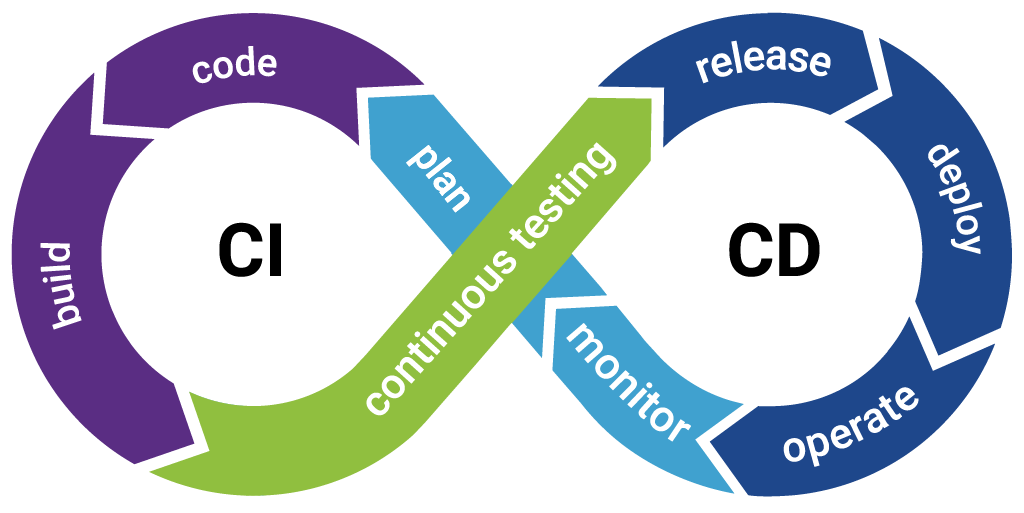
\includegraphics[width=10cm]{ci-cd-diagram}
    \centering
\end{figure}
\subsection{Continuous Integration}
The concept of Continuous Integration was first coined by Grady Booch in 1991, but became mainstream with the rise of eXtreme Programming in 1999. The reference book on the topic is \Citeauthor{Duvall2007}'s ``Continuous Integration: Improving Software Quality and Reducing Risk'' that was published in 2007.

Continuous Integration centers around methods of automating the integration of code changes from various contributors into a single software project is known as continuous integration (CI). It's a fundamental DevOps best practice that enables developers to merge code changes into a single repository regularly, after which builds and tests are executed. Before integration, the new code is checked for correctness using automated tools.
\subsection{Continuous Delivery}
Getting code integrated is not enough, eventually it only provides value in the hands of users so it needs to be deployed and end up in a production environment eventually. Continuous Delivery is the capacity to swiftly and reliably deploy updates of all kinds, such as new features, configuration modifications, bug fixes, and experimentation, into production or to the customer.

In 2010, \Citeauthor{Humble2010} and David Farley published their milestone book ``Continous Delivery, Reliable Software Releases through Build, Test, and Deployment Automation''. This book brings an extended view on process, practices and tools required to get to scalable deployments.

In 2021, \Citeauthor{Farley2021} published a sequel book on the topic titled ``Continuous Delivery Pipelines: How To Build Better Software Faster''. it is a quick read full of practical tips to get started with Continuous Delivery.

The objective is to make deployments predictable, routine tasks that can be carried out on demand, including a large-scale distributed system, a complex production environment, an embedded device, or an app.

All of this is made possible by our commitment to keeping our code deployable, even in the face of everyday modifications made by teams of hundreds or sometimes thousands of developers. As a result, we do away with code freezes and the integration, testing, and hardening phases that typically come after "dev complete".

\begin{figure}[!h]
    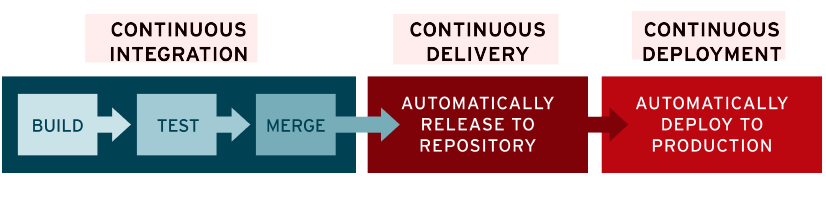
\includegraphics[width=10cm]{ci-cd-flow-desktop_edited_0}
    \centering
\end{figure}
\section{Metrics}
\label{sec:metrics}
Although the project methodology at Showpad centers around \gls{Scrum}, where Velocity is the classic metric to monitor productivity, management uses the traditional lean metrics instead. Before zooming in to the metrics, we set the methodological context in this literature study.
\subsection{Lean Software Development}
There is a lot of literature on measuring team performance and productivity in a software development context. Providing a complete spectrum overview of all methodologies and their related metrics would lead us too far. We focus on the process and its metrics applied at Showpad and will provide the background on these metrics in this literature study.
At Showpad, the core of the metrics set used by management to monitor and control productivity boils down to the lean metrics of \gls{Cycletime}, Throughput, and Work In Progress. 
\newline
\newline
Lean software metrics build on the industrial production methodology called the Toyota Production System. Unlike the design and mass production of physical products, designed by engineers and produced by machines in factories, the design, creation, maintenance, and evolution of software products are fundamentally different, so the usage of lean methodologies and metrics have to be tuned towards this other reality.
\newline
\newline
In their 2007 book ``Implementing Lean Software Development: From Concept to Cash''  \Citeauthor{Poppendieck2007} give an excellent overview of how the lean concepts and practices in manufacturing translate to the world of software development. In Chapter 5 of the book, they zoom in on the theme of speed and time to value, bringing us to the core lean metrics: \gls{Cycletime}, Throughput, and Work In Progress. The mathematical relationship between those three core metrics is illustrated by explaining Little's Law.
\newline
\newline
In his  2018 book ``Project to Product, how to survive and thrive in the age of digital disruption with the flow framework'', \Citeauthor{Kersten2018} builds further on the lean legacy. Based on his analysis of the manufacturing practices observed in the Leipzig BMW plant, he looks for the commonalities and differences between modern lean-based car production processes and procedures and their software development counterparts. In his book, Kersten describes the epiphanies he encountered throughout his research. His 3rd epiphany, ``Software value streams are not linear manufacturing processes but complex collaboration networks that need to be aligned to products'' goes to the fundamental difference between applying lean in the manufacturing context versus the software development context. In a previous section of this chapter, we zoomed in on state of the art on Architectural patterns as they are applied at Showpad. Kersten's first epiphany, ``Software productivity declines and thrashing increases as software scales, due to disconnects between the architecture and the value stream.'' connects the dots and helps understand how architectural choices influence the productivity in a software organization.
\subsection{Lean Metrics and Flow}
Where Poppendieck's and Kersten's books put the lens on the lean software development methodology, another great book zooming into the lean metrics is the book titled  ``Actionable Agile Metrics for Predictability, and introduction'' by \Citeauthor{Vacanti2015}. This book solely focuses on core lean metrics, zooms in on the relationship defined by Little's law, and elaborates on the concept of flow. It also deep dives into continuous flow diagrams to illustrate and analyze flow.
\subsection{Little's Law} 
Little's Law is a queueing theorem by John Dutton Conant Little. The formula is streight forward: \begin{math}L = \lambda * W \end{math}.
Where \begin{math}L \end{math}
 is the average number of items in the queueing system.
 \begin{math} \lambda \end{math}  
 is the average number of items arriving per unit of time. And 
 \begin{math}W \end{math} 
 is the average wait time in the system for 1 item.
\newline
\newline
In the software development context, the ``item'' is a unit of work. As mentioned in the Introduction chapter, in Showpad, there are two granularity levels when thinking about work units. An \gls{Epic} is the top-level units of work, all Epics together composing the Roadmap. Epics are typically delivered in 1 release cycle. An \gls{Epic} is further broken down into several User Stories. A user story is generally delivered in 1 sprint. A user story is the unit of work for one \gls{Scrum} team. So when we want to get a view of the productivity of a \gls{Scrum} team, the Item in Little's Law formula is a user story.
\newline
\newline
In chapter 3 of his book, Vacati translates Little's law to the three lean metrics.
\newline
\newline
Average \gls{Cycletime} = Average Work In Progress / Average Throughput
\newline
\newline
\subsection{Cycle Time}
From a business perspective, the core question \gls{Cycletime} answer is: How long (elapsed time) will the promised work take to complete?
\newline
\newline
\Gls{Cycletime} is the elapsed time from the start of the first task to finishing the last job to deliver 1 item. In the context of a \gls{Userstory}, the clock starts ticking when anyone starts working on the \gls{Userstory} until the last task to deliver the \gls{Userstory} is finished. When evaluating \gls{Cycletime} in the context of an \gls{Epic}, the clock starts ticking when anyone starts working on the first \gls{Userstory} until the last \gls{Userstory} to deliver the \gls{Epic} is finished.
\newline
\newline
Important to mention is that \gls{Cycletime} includes both value-added time (people actively working on tasks) and non-value-added time (waiting time, for example).
\newline
\newline
According to Little's Law: \gls{Cycletime} = Work In Progress / Throughput
\newline
\newline
In the context of Showpad, management talks about Lead Time instead of \gls{Cycletime}. Lead Time and \gls{Cycletime} are two terms that get regularly mixed up. In manufacturing, the distinction is more straightforward. \Gls{Cycletime} covers an individual process step, while Lead Time covers the entire process. As delivering a piece of software takes multiple process steps, even on \gls{Userstory} level, there is the tendency to use the term Lead Time instead of \gls{Cycletime}. As both terms share the same formula but mainly differ on scope level, and for simplicity's sake, we will stick to the usage of \gls{Cycletime} throughout this thesis.
\subsection{Throughput}
From a business perspective, the core question "Throughput" answer is: How many features can I expect?
\newline
Throughput is the ultimate productivity metric. It indicates how many work items we can deliver in a period of time. Translated to the context of Showpad, how many user stories can we deliver in 1 \gls{Sprint}, and how many \glspl{Epic} can we deliver in 1 release cycle.
\newline
\newline
According to Little's Law: Throughput = Work In Progress / \gls{Cycletime}
\newline
\subsection{Work In Progress}
Work In Progress (WIP) equals the number of work items that are worked on in parallel. 
\newline
\newline
Work In Progress does not line up with a direct customer question in business, but it is one of the most influential metrics regarding flow. And limiting Work in Progress is one of the most effective ways to minimize \gls{Cycletime} and maximize Throughput.
\newline
\newline
According to Little's Law: Work In Progress = \gls{Cycletime} * Throughput

%%=============================================================================
%% Methodologie
%%=============================================================================

\chapter{\IfLanguageName{dutch}{Methodologie}{Methodology}}
\label{ch:methodologie}

%% TODO: Hoe ben je te werk gegaan? Verdeel je onderzoek in grote fasen, en
%% licht in elke fase toe welke stappen je gevolgd hebt. Verantwoord waarom je
%% op deze manier te werk gegaan bent. Je moet kunnen aantonen dat je de best
%% mogelijke manier toegepast hebt om een antwoord te vinden op de
%% onderzoeksvraag.
\section{Exploring Opportunities}
Showpad is a continuously growing company, as both the employee count enlarges, so do the codebases of the different teams and applications. With scalability in mind, as said in the state-of-the-art chapter, monorepos (which Showpad currently uses) aren’t really optimal to scale up to the point of the currently enormous codebases within the company. 
\subsection{Developer's Productivity}
Witnessing first hand the CI/CD pipelines, test and build times. The queueing  and waiting for the frontend monolith CI/CD pipeline to finish and get your changes deployed in production or not - in case code is rolled back - have a substantial impact on the productivity of engineers accross the 18 scrum teams. These are real pain points for developers and can become frustrating over time. Having identified the problem and having heard about the scalability potential of Micro Frontends the goal was set. Trying to transform some part of the main Showpad web application into a Micro Frontend application.
\subsection{Ambitious but acchievable Goal}
Although the potential of microfrontends goes wider than developer's productivity, selecting a realistic scope for a proof of concept in the context of this Bachelor Thesis was important. As this was also the first experiment with micro frontends across Showpad, there was a strong interest from within the front-end guild to try and prove that a Micro Frontend architecture is more efficient and more scalable than the current monolithic structure and providing developers a better developer experience through significantly improved build times and less waiting on the pipeline before merging and deploying.
\section{Knowledge building}
An important part of the methodology was conducting literature study and research on the current state of the Showpad product architecture, and learning about the architectural concepts that come with micro frontends. Next to reading articles, watching videos and reading books on the different topics as mentioned in \autoref{ch:stand-van-zaken}, I had the opportunity to participate in a video meeting with Luca Mezzalira, the authority and author on Microfrontends.
\section{Setting the scope of the Proof Of Concept}
With the goal of this proof-of-concept in mind, the knowledge about Micro Frontends and how to extract and implement them still had to be acquired. There was a small newly created initiative around Micro Frontends by a couple of members of the frontend guild. With the help of them the project got started. 
\section{Isolating the microfrontend application}
A part of the Showpad web application was decided on to isolate and transform into the Micro Frontend. The first big struggle was getting the application extracted out of the highly dependant structure that is the frontend monorepo.

After this problem was dealt with, the Micro Frontend application could be run on its own. Started some tests on how efficient the application ran by itself. There were still some challenges to resolve, some dependencies that were still missing or Angular errors that were pretty vague and wasted a lot of time on on finding out what was wrong. With most errors out of the way the host application (the main Showpad web application) got prepared for the remoteEntry point of our Micro Frontend application. 

After facing some more issues with the integration of the remote application into the host application we ran into another problem. Deciding on how we were going to merge and deploy our application without affecting everyone else in the application. So we decided on creating a feature flag in “Central Station” (the PHP based back-end). With this feature flag in place every developer within Showpad could choose to turn this on or off. Of course this feature flag had to get the functionality to either turn on or off the Micro Frontend application. So a routing orchestration was built into the host application. If the feature flag is turned on the Micro Frontend version of our application would be run and the web application is routed to the remote entry. If the feature flag is turned off Micro Frontend application does nothing and the web application gets routed to the same place it has always been routed to.
\section{Continuous Integration substantially improved}
The applications both work fine and build times have improved over 400\%. Although my time at Showpad ran out and we had not figured out yet how to deploy this to production and we did not find out how our application had an effect on the CI/CD pipeline. But we continued after the end of my internship. The proof-of-concept is running on the staging environment of Showpad.
\section{Running the proof-of-concept}
In this proof-of-concept we are facing some major business architectural difficulties to really show the potential of micro frontends. First off in an ideal micro frontend architecture the entirety of the Showpad developer teams should be taken under the loop, to check if all teams are still having to work on the same business areas. As for this micro frontend proof-of-concept, there weren’t any architectural changes to the whole of the codebase or the teams but rather isolating one particular part of the main application and transforming it into a micro frontend and transforming the main application to a shell application which should host all micro frontends inside.

The entire proof-of-concept project is running on Showpads staging environment hidden behind a feature flag. A feature flag is something used to enable or disable certain features of the application for certain users so that not everyone is affected by these changes to the application.



\chapter{\IfLanguageName{dutch}{Uitgangspunt}{Baseline}}
\label{ch:baseline}
\section{Technology Stack}
The main technologies used at team CRM are Angular using NgRx for the frontend developers, Kotlin for the newer backend and PHP on the legacy backend. Something about AWS for the backend but no clue hoe dat in elkaar zit.

\section{Architecture}
\subsection{Monorepo}
The frontend of the main web application from Showpad is stored in one big mono repo,
millions of lines of code all in one massive repository.
\section{CI/CD reality}
There are a lot of checks every time there is an merge request ready to get merged into Master.
All of these checks take a lot of time to be run through. Here comes the term “pipeline babysitting” from.

Because it’s a monorepo there are many things that can go wrong, as mentioned before and shown in the screenshot there are a lot of checks thus a lot of potential for one of them to fail. End-to-end tests take the most amount of time to run through. Stated by some colleagues the pipeline is very well organized but because of the enormous codebase it takes a lot of time to get through.

Having witnessed the pipeline myself it takes a really long time for even the smallest changes to the code. But there is light at the end of the tunnel because the pipeline is in constant improvement and there are a couple of experiments with architecture going on like this proof-of-concept to try and improve these wait times.

\begin{figure}[!h]
    \centering
    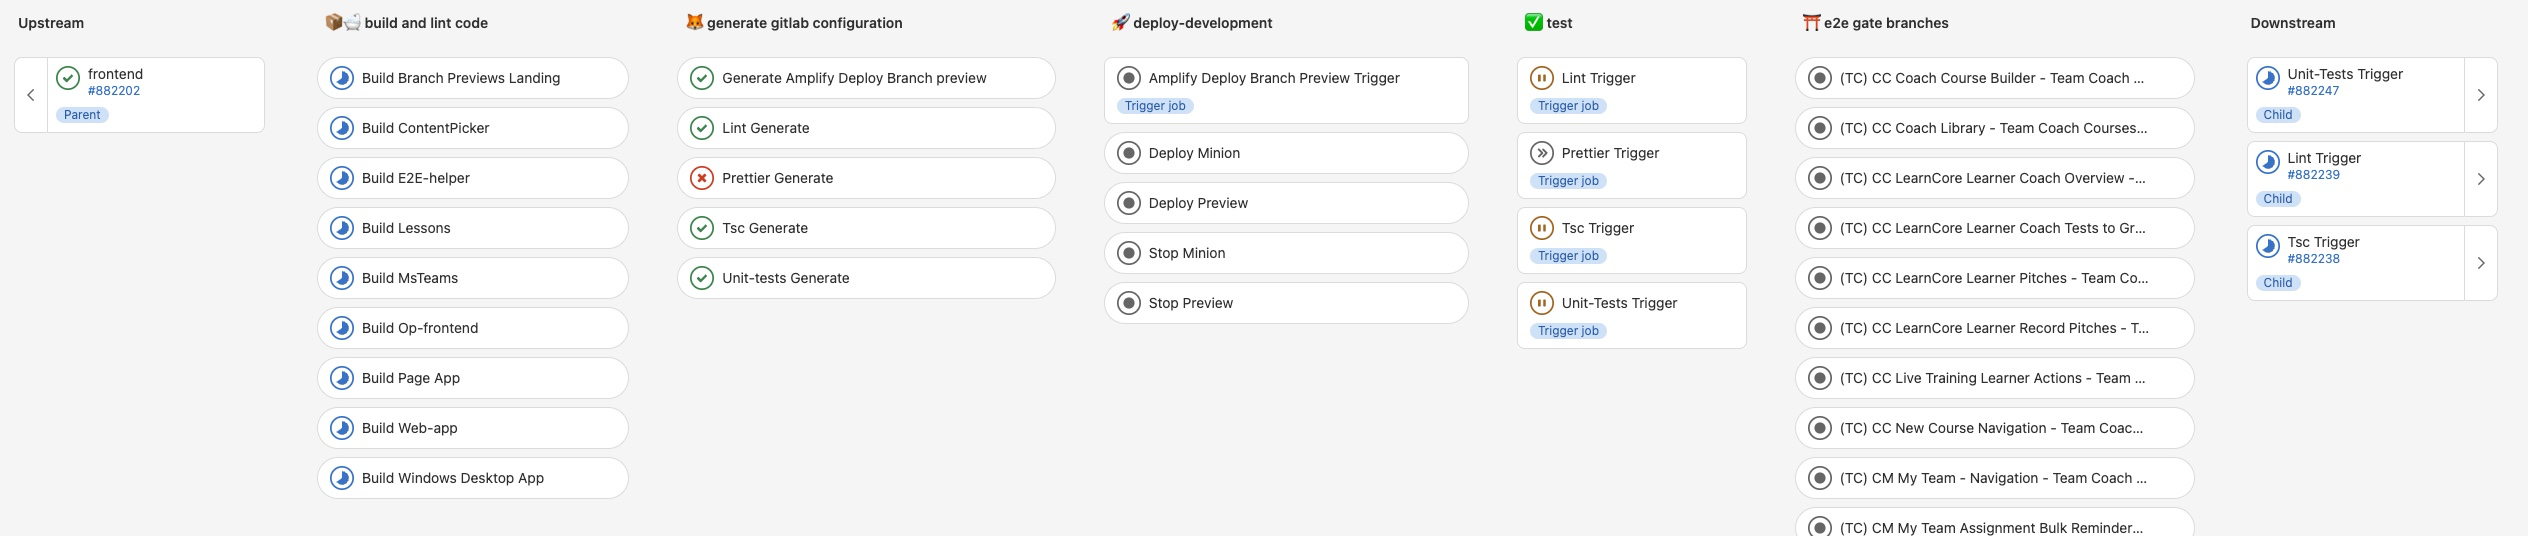
\includegraphics[width=15cm]{pipeline}
    \caption{Screenshot of current pipeline within Showpad}
\end{figure}

\section{Metric baseline}
\subsection{Build times}
If a developer wants to test his changes locally, he needs to build the entire Showpad web application. This takes on average 4 minutes and 11 seconds. Which can be frustrating to wait four minutes to just spin up the application.

\subsection{CI/CD pipeline runtime}
In the current CI/CD it sometimes takes hours to just run through the pipeline, this is mainly caused by the end-to-end tests. The pipeline without the end-to-end tests takes on average 35 minutes and 29 seconds which on its own is not that bad. The pipeline is constantly being improved so the time waiting on the pipeline is still getting better.

\subsection{Cycle Time}
The biggest problem in the cycle time in the monorepo structure is the dependability of teams on each other. They always have to wait for their code to be deployed to production, which currently happens about twice a day. A simplified version of the current process to get code into production is shown in figure 4.2.

\begin{figure}[!h]
    \centering
    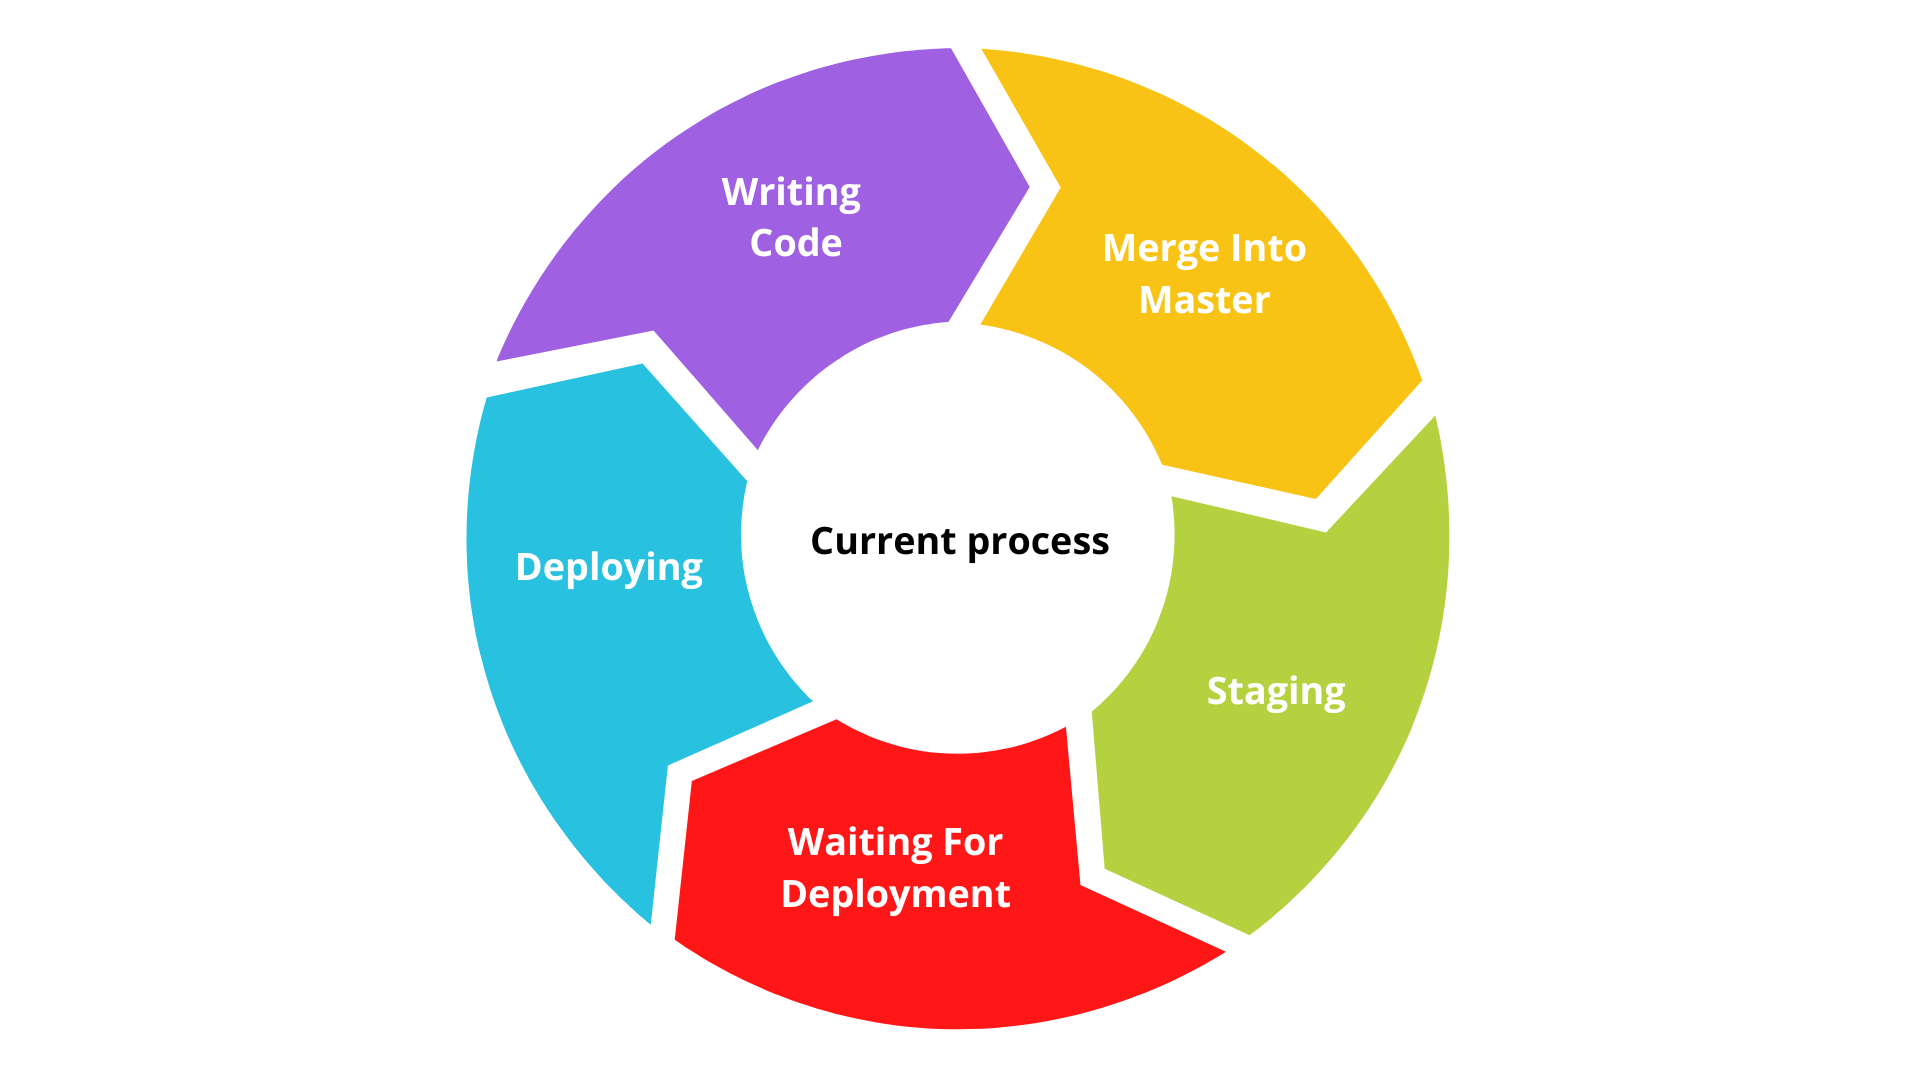
\includegraphics[width=12cm]{current-cycle}
    \caption{Simplified current process for getting code into production}
\end{figure}

\chapter{\IfLanguageName{dutch}{Scope Micro-Frontend App}{Scope Micro-Frontend App}}
\label{ch:scopemicrofrontendapp}
\section{Functional Scope}
The functional scope of this proof-of-concept is split up into two parts. The first part being the micro frontend or remote application and the second part is the shell application the remote application will be run in.

The shell application in our case is the main Showpad web application. The remote application chosen to be isolated and transformed is known as the CRM widget (shown in figure 5.1). The functionality of this CRM widget is to get all the recommended sales content that is assigned to the logged in account. With this widget the sales representatives have easy access to their content and are able to quickly view statistics of their content, share it or simply open and use their content.

\begin{figure}[!h]
    \centering
    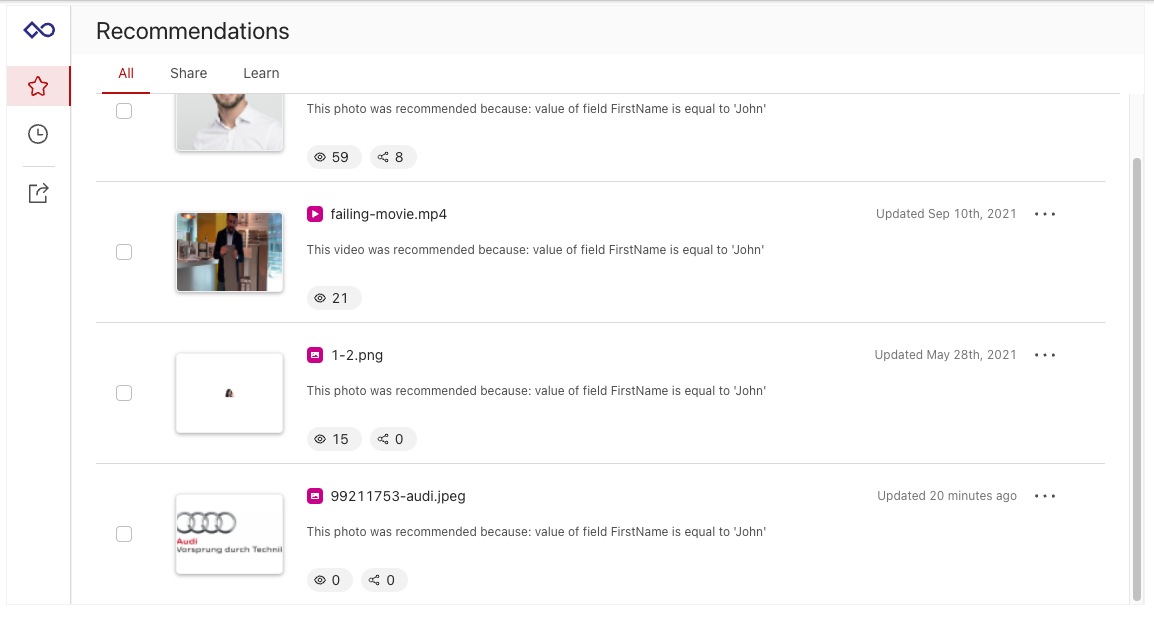
\includegraphics[width=12cm]{crm-widget}
    \caption{CRM widget}
\end{figure}

\section{Steps to Extract}
Decoupling the existing application
Setting up the environment
Running application on different port
Feature flag in central station to hide the mfe behind
Fixing stuff until it worked
\section{Challenges}
Following conventions and fitting it to our needs
Merging changes into master
Dependency issues, forgetting to import some dependencies
Setting it up for testers

The main challenge was because we are using a monorepo architecture and we’re trying to decouple parts/libraries from this highly dependent structure…
what does it mean in practice for our case:
dependencies -> for example asset viewer, external modules (npm modules), application state/store, authorisation
feature flag/routing -> deciding the convention to be used by the company for this purpose… either with different routes and guards or going against the best practices and hacking the route
keeping up with the metamorphosis of the monorepo… all the changes coming from master related or not with micro front ends
all of the unknown errors which we came to discover while running it… a major part was very vague from angular side.

\chapter{\IfLanguageName{dutch}{Resultaat}{Results}}
\label{ch:results}
\section{Metric outcome}
In this thesis we are measuring a couple of factors to see what the improvements are using micro frontends as opposed to the currently in place monorepo.

\subsection{Improvements for the developer}
Starting with the simplest to measure metric, the build times between the applications.
This metrics shows how much faster the micro frontend application builds and is ready to be tested by the developer. In our measures of building the CRM widget micro frontend application about 10 times, the average build speed is about 1 minute and 3 seconds. When the web application is built this takes about 4 minutes and 11 seconds on average. Seeing this there is an improvement of nearly 400\%. This means developers have to wait only a fourth of the time that they are used to and will be way faster in getting to test their written code.

\begin{table}
    \centering
    \begin{tabular}{|c|c|}
        \hline
        & Average build time \\ [1ex] 
        \hline\hline
        Monorepo & 4' 11'' \\  [1ex]
        \hline
        Micro Frontend & 1' 2'' \\[1ex]
        \hline
        Difference & 3' 8''  \\ [1ex] 
        \hline
        \multicolumn{2}{| c |}{Performance improvement of 400\%}\\
        \hline
    \end{tabular}
    
    \caption{Build times}
\end{table}

\subsection{Improvements for CI/CD}
As the pipeline for the micro frontend application was not finished yet, a simulation was made to get an idea of what the improvements would be in pipeline finishing speeds. The pipeline that is in place nowadays runs and tests the whole application as opposed to the future pipeline that would only run those checks for the specific micro frontend application. For this simulation a closer look was taken at all the pipeline checks and only those that were relevant to the micro frontend application were kept when the pipeline was run. The end-to-end tests were also excluded from both pipelines because they take the longest and will be removed in the future anyways. Of course this is not a 100\% accurate representation of what the true potential is in the future. But with our simulation we can already see some improvements.

The average time it takes for the entire pipeline with all its checks, tests, build and deploy times is 35 minutes and 29 seconds. The pipeline customized for the micro frontend application takes an average of 27 minutes and 51 seconds. As the data shows this is already an improvement of 7 minutes and 38 seconds. This accounts for an improvement of 27\%. Since the micro frontend initiative is still new within Showpad those times can still drastically improve. This simulation shows already good improvement but the true potential will be shown in the future when the actual pipeline is finished.

\begin{table}
    \centering
    \begin{tabular}{|c|c|c|c|}
        \hline
         & Tests \& Checks & Build \& Deploy & Total time \\ [1ex] 
        \hline\hline
        Monorepo & 21' 26'' & 14' 03`` & 35' 29`` \\ [1ex]
        \hline
        Micro Frontend & 17' 34`` & 10' 17`` & 27' 51`` \\[1ex]
        \hline
        Difference & 3' 52`` & 3' 46`` & 7' 38`` \\ [1ex] 
        \hline
         \multicolumn{4}{| c |}{Performance improvement of 27\%}\\
         \hline
    \end{tabular}
   
    \caption{Time to complete the CI/CD pipeline}
\end{table}

\subsection{Improvements in cycle time}
The most important metric is towards the user of the product. So how much has the micro frontend architecture an effect on how fast the user can have his hands on new features and fixes. 

For this metric it is important to understand that the currently main time losing factor within the process of getting code to production is being dependent on other teams. Since the current process of getting code to production is:

\begin{enumerate}
\item Writing code
\item Merging it into master through the pipeline
\item Testing in a staging environment
\item Waiting for one of the two deployments a day into production
\item Deploying
\end{enumerate}

Step 4 is the biggest time waster since all teams have to wait to deploy their code together. Deployments are currently scheduled to happen twice a day for the entire Showpad web application. In a micro frontend environment this wait time is completely eliminated because teams are no longer dependent on each other. Every team has their own micro frontend application which can be deployed to production whenever the team is ready to do so. So a team could hypothetically deploy 16 times a day if they really wanted to. This improves the cycle time so immensely it would not even be comparable.

\begin{figure}[!h]
    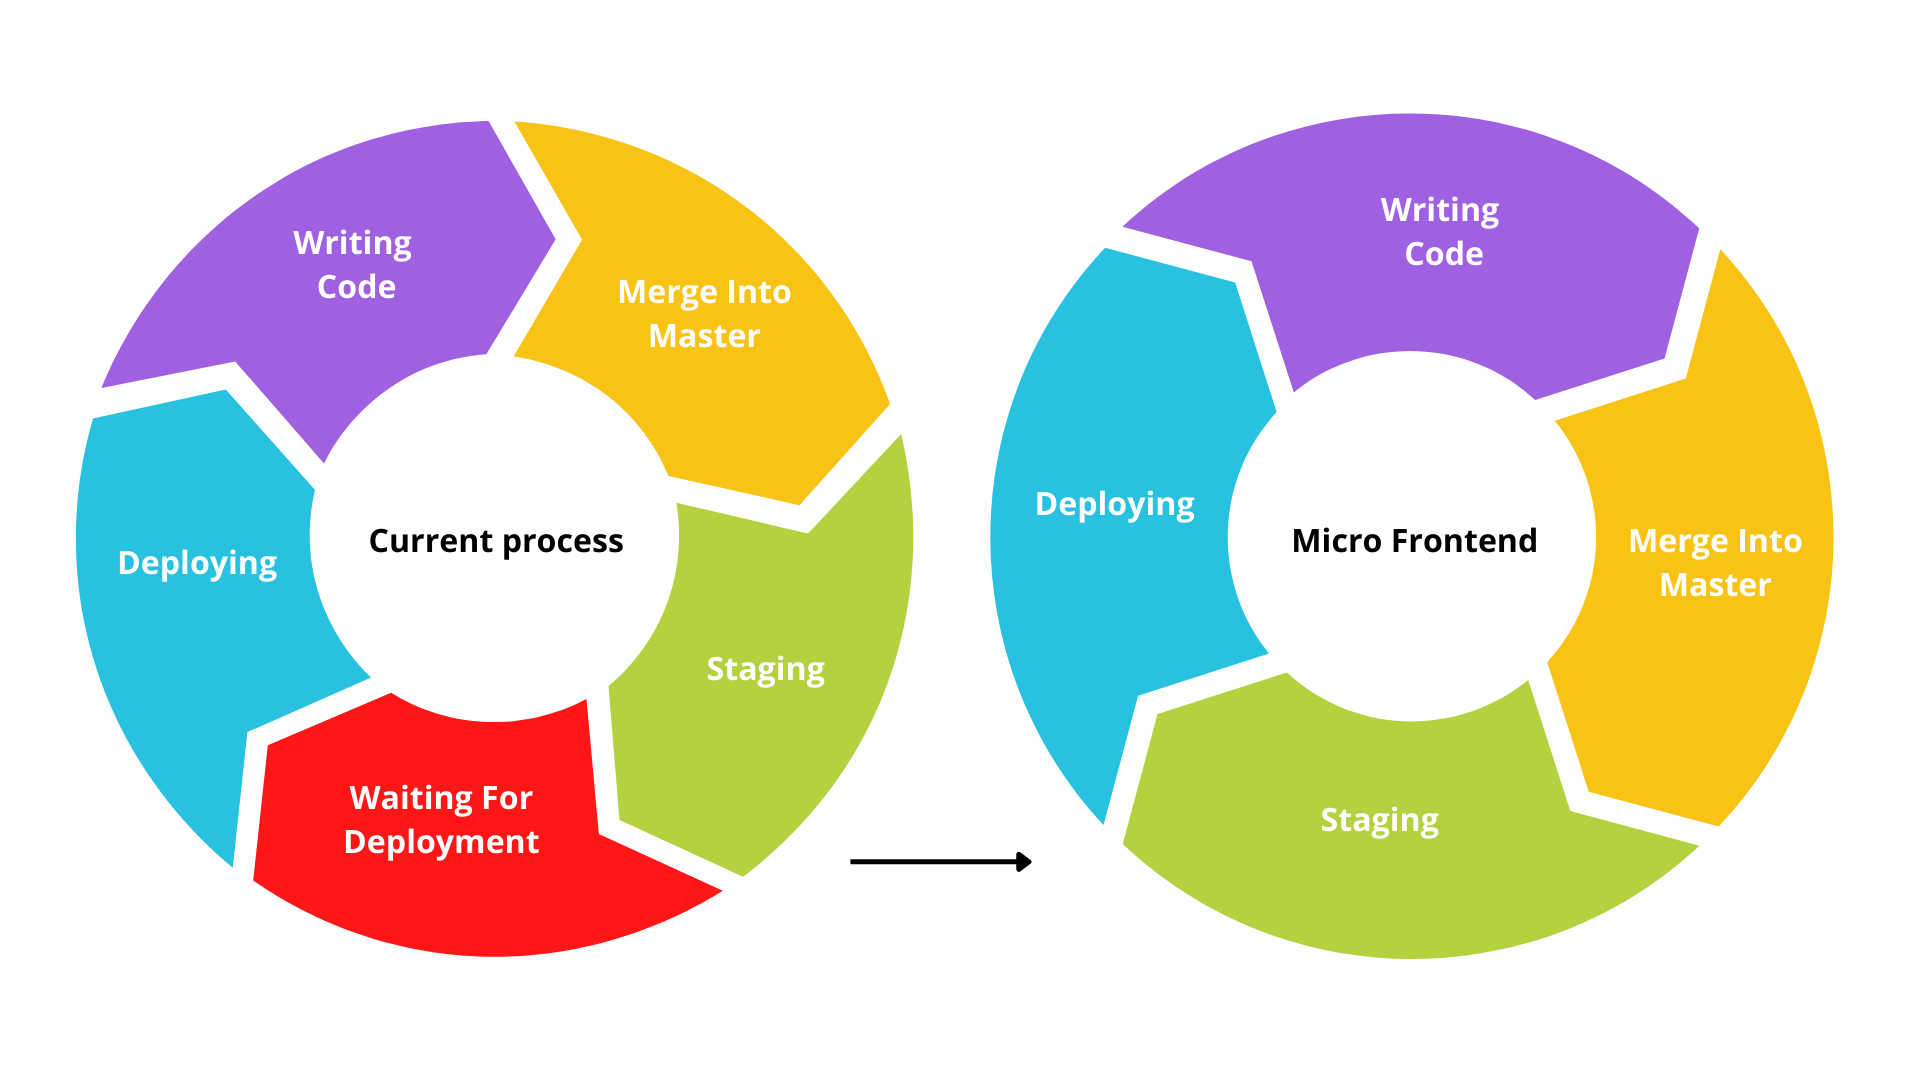
\includegraphics[width=12cm]{cyclus}
    \centering
\end{figure}

%%=============================================================================
%% Conclusie
%%=============================================================================

\chapter{Conclusion}
\label{ch:conclusie}

% TODO: Trek een duidelijke conclusie, in de vorm van een antwoord op de
% onderzoeksvra(a)g(en). Wat was jouw bijdrage aan het onderzoeksdomein en
% hoe biedt dit meerwaarde aan het vakgebied/doelgroep? 
% Reflecteer kritisch over het resultaat. In Engelse teksten wordt deze sectie
% ``Discussion'' genoemd. Had je deze uitkomst verwacht? Zijn er zaken die nog
% niet duidelijk zijn?
% Heeft het onderzoek geleid tot nieuwe vragen die uitnodigen tot verder 
%onderzoek?
Reducing the lead time "from idea till smile of the customer" is a frequently stated quote at Showpad, indicating the importance of getting product innovation in the hands of customers and users as soon as possible.

Core to the value proposition from a micro frontend architecture is that it will substantially shorten the cycle time of every team by eliminating the need for teams to depend and wait on each other to deploy. Each team takes full code ownership and can choose to deploy whenever they want. This will result in users getting new products and features faster. Besides this considerable upside for customers, the developer experience improves drastically through the reduced build and CI/CD pipeline runtimes.

In this bachelor thesis, we evaluated the potential of how the micro frontend architecture pattern can contribute to the productivity of developers and teams and how it contributes to the reduction in cycle time. 

The results of the proof of concepts show a positive impact. The isolated functionality's build time was four times faster than the baseline measurements. The cycle time of the adapted CI/CD pipeline for the micro frontend application was reduced by 27\%.

These results for sure look promising. It has the potential for the productivity of individual developers and teams as to the autonomy of teams in a multi-team development organization like Showpad. 

But it will not come for free. 

It is known that in microservice and micro frontend architectures, the system's complexity increases due to the growing number of components. 

Secondly, decomposing a monolith architecture requires a lot of work, and it will take time before the full impact materializes. 

Last but not least, decomposing a monolith architecture is not only a technical challenge but requires alignment to the product domain model. To get to this alignment, thought leaders in microservice and micro frontend architectures plea for applying Domain Driven Development as the basis.

A software company's primary purpose is to get product innovation in the hands of customers and users as soon as possible. In Showpad, it is now up to the Product \& Engineering leadership to further explore the usage of Micro frontends to answer the architectural challenges that influence scaling the product and the autonomy and productivity of teams.

This project was a fun proof-of-concept to work on. I acquired a lot of new knowledge about different architectures and their advantages and drawbacks, as well as know-how and conventions using Angular, NgRx, and module federation.


%%=============================================================================
%% Bijlagen
%%=============================================================================

\appendix
\renewcommand{\chaptername}{Appendix}

%%---------- Onderzoeksvoorstel -----------------------------------------------

\chapter{Onderzoeksvoorstel}

Het onderwerp van deze bachelorproef is gebaseerd op een onderzoeksvoorstel dat vooraf werd beoordeeld door de promotor. Dat voorstel is opgenomen in deze bijlage.

% Verwijzing naar het bestand met de inhoud van het onderzoeksvoorstel

%\externaldocument{./voorstel/baeyens_simon_microfrontends}
%---------- Inleiding ---------------------------------------------------------

\section{Introduction} % The \section*{} command stops section numbering
\label{sec:introductie}

Micro frontends have been on the rise in recent years and I was intrigued by the idea of structuring one application into many smaller applications which all work together. Since Showpad is a scale-up organisation it is only right to try and prove the scaling potential of the micro frontend architecture and its many other benefits for the developers themselves. Nobody likes long build times when they are trying out their code so here is also a lot of promise in improving these non productive wait times significantly.

%---------- Stand van zaken ---------------------------------------------------

\section{State-of-the-art}
\label{sec:state-of-the-art}

\subsection{What are Micro Frontends?}
Micro-Frontend applications are an architecture inspired by the microservices architecture.
In this kind of architecture monolithic codebases are broken down into many smaller “applications” which all work together as if it is one big application. 

\subsection{Why use Micro Frontends?}
The main advantages of Micro Frontends are its scalability, the possibility to adopt different technologies and its development efficiency (faster build/runtimes).

\subsection{What is a monolithic architecture?}
In a monolithic architecture the application is structured unifiedly so that the codebase is all in one place.

\subsection{Why use a monolithic structure?}
The main advantage of using a monolithic structure is its simplicity in many different aspects. All the code of the application is in one place so everything is straight-forward and there is no additional architectural knowledge required.

\subsection{What is CI/CD?}
CI/CD or Continuous Integration / Continuous Delivery is a method where applications are being delivered to the customer by using a form of automation at different stages of development.
The goal of Continuous integration is that the application is always in a working state by checking if the code works before it gets pushed into production using automated tests.
The goal of Continuous delivery is to make sure that the new changes are merged in correctly with the already  existing code in production and still is in a working state.


%---------- Methodologie ------------------------------------------------------
\section{Methodologies}
\label{sec:methodologie}

The first step of the process was researching and understanding both architectures.
Following steps of this proof-of-concept and comparative study is to work and test how the monolithic architecture behaves also to get familiar with the codebase. The next step is choosing and isolating one part of the whole application and transforming it into a micro frontend. After this is done the real world comparison can start. Checking the performance of both architecture and also if the hoped for potential is fulfilled.

%---------- Verwachte resultaten ----------------------------------------------
\section{Expected results}
\label{sec:verwachte_resultaten}

The result of this thesis should be a proof-of-concept within Showpad to test if the micro frontend architecture is beneficial to the workflow of the developers and the CI/CD.
Expectations are that the developers could work more efficiently through the benefits of the architecture's build time speeds, full code ownership for every team and own deployments.

%---------- Verwachte conclusies ----------------------------------------------
\section{Expected conclusions}
\label{sec:verwachte_conclusies}

Both architectures will both have its pros and cons but in the end the micro frontend architecture looks more applicable to Showpad because of the architectures potential of scalability. Since Showpad is a continuously growing organisation where new teams are created regularly.


%%---------- Andere bijlagen --------------------------------------------------
% TODO: Voeg hier eventuele andere bijlagen toe
%\input{...}

%%---------- Referentielijst --------------------------------------------------
\printbibliography[heading=bibintoc]

\end{document}
